\documentclass{article}

\usepackage[margin=1in]{geometry}
\usepackage[colorlinks,linkcolor=blue,filecolor=blue,citecolor=magenta,urlcolor=blue]{hyperref}
\usepackage{bm,amsmath,amsthm,amssymb,multicol,algorithmic,algorithm,enumitem,graphicx,subfigure}
\usepackage{xargs}
\usepackage{natbib}
\usepackage{stmaryrd}


\def\M{\mathcal{M}}
\def\A{\mathcal{A}}
\def\Z{\mathcal{Z}}
\def\S{\mathcal{S}}
\def\D{\mathcal{D}}
\def\R{\mathcal{R}}
\def\P{\mathcal{P}}
\def\K{\mathcal{K}}
\def\E{\mathbb{E}}
\def\F{\mathfrak{F}}
\def\l{\boldsymbol{\ell}}

\newtheorem{Fact}{Fact}
\newtheorem{Lemma}{Lemma}
\newtheorem{Prop}{Proposition}
\newtheorem{Theorem}{Theorem} 
\newtheorem{Def}{Definition}
\newtheorem{Corollary}{Corollary}
\newtheorem{Conjecture}{Conjecture}
\newtheorem{Property}{Property}
\newtheorem{Observation}{Observation}
\newtheorem{Exa}{Example}
\newtheorem{assumption}{H\!\!}
\newtheorem{Remark}{Remark}
\newtheorem*{Lemma*}{Lemma}
\newtheorem*{Theorem*}{Theorem}
\newtheorem*{Corollary*}{Corollary}
 
\newcommand{\eqsp}{\;}
\newcommand{\beq}{\begin{equation}}
\newcommand{\eeq}{\end{equation}}
\newcommand{\eqdef}{\mathrel{\mathop:}=}
\def\EE{\mathbb{E}}
\newcommand{\norm}[1]{\left\Vert #1 \right\Vert}
\newcommand{\pscal}[2]{\left\langle#1\,|\,#2 \right\rangle}
\def\major{\mathsf{M}}
\def\rset{\ensuremath{\mathbb{R}}}


\begin{document}



\title{AniLA: Anisotropic Langevin Dynamics for training Energy-Based Models}

 \author{\textbf{Belhal Karimi, Jianwen Xie, Ping Li} \\\\
 Cognitive Computing Lab\\
 Baidu Research\\
   10900 NE 8th St. Bellevue, WA 98004, USA
 }

\date{}
\maketitle

\begin{abstract}
We develop in this paper
\end{abstract}

\section{Introduction}
The modeling of a data generating process is critical for many tasks.
A growing interest in generative models within the realm of computer vision has led to multiple interesting solutions.
In particular, Energy Based Models (EBM) \citep{zhu1998filters,lecun2006tutorial}, are a class of generative models that learns high dimensional and complex (in terms of landscape) representation/distribution of the input data.
Since inception, EBMs have been used in several applications including computer vision \citep{ngiam2011learning, xie2016theory,xie2020generative,du2019implicit}, natural language processing \citep{mikolov2013distributed,deng2020residual},  density estimation \citep{wenliang2019learning,song2020sliced} and reinforcement learning \citep{haarnoja2017reinforcement}.

Formally, EBMs are built upon an unnormalized log probability, called the energy function, that is not required to sum to one, as standard log probability functions.
This noticeable feature allows for more freedom in the way one parametrizes the EBM.
For instance, Convolutional Neural Network (CNN) can be employed to parametrize the energy function, see \citep{xie2016theory}.
Note that this choice is highly related to the type of the input data, as mentioned in \citep{song2021train}.

The training procedure of such models consists of finding an energy function that assigns to lower energies to observations than unobserved points.
This phase can be casted into an optimization task and several ways are possible to achieve it.
In this paper, we will focus on training the EBM via Maximum Likelihood Estimation (MLE) and defer the readers to \citep{song2021train} for alternative procedures.
Particularly, while using MLE to fit the EBM on a stream of observed data, the high non-convexity of the loss function leads to a non closed form maximization step. In general, gradient based optimization methods are thus used during that phase.
Besides, given the intractability of the normalizing constant of our model, the aforementioned gradient, which is an intractable integral, needs to be approximated.
A popular and efficient way to conduct such approximation is to use Monte Carlo approximation where the samples are obtained via Markov Chain Monte Carlo (MCMC) \citep{meyn2012markov}.
The goal of this embedded MCMC procedure while training the Energy-based model is to synthesize new examples of the input data and use those new synthetic observations, in our case images, to approximate some expectations that we will describe later.
The sampling phase is thus crucial for both the EBM training speed and its final accuracy in generating new samples.

The computational burden of those MCMC transitions at each iteration of the EBM training procedure is alleviated via different techniques in the literature.
For instance, in \citep{nijkamp2019learning}, the authors develop a short-run MCMC as a flow-based generator mechanism despite its non convergence property.
A large class of solutions aiming at reducing the cost of running MCMC until convergence, which in practice can be unfeasible, is using Contrastive Divergence \citep{hinton2002training} and persistent Contrastive Divergence \citep{tieleman2008training}.
This principled approach keeps in memory the final chain state under the previous global model parameter and uses it as the initialization of the current chain.
The heuristic of such approach is that along the EBM iterations, the conditional distributions, depending on the model parameter, are more and more similar and thus using a good sample from the previous chain is in general a good sample of the current one.
Though, this method can be limited during the first iterations of the EBM training since when the model parameter changes drastically, the conditional distributions do too and samples from two different chains can be quite inconsistent.
Several extensions varying the way the chain is initialized can be found in \citep{welling2002new,gao2018learning,du2019implicit}.

An interesting line of work in the realm of MCMC-based EBM tackles the biases induced by stopping the MCMC runs too early. 
Indeed, it is known, see \citep{meyn2012markov}, that before convergence, MCMC samples are biased and thus correcting this biase while keep a short run and less expensive run is an appealing option.
Several contributions aiming at removing this bias for improved MCMC training include coupling MCMC chains, see \citep{qiu2019unbiased,jacob2020unbiased} or by simply estimating this bias and correct the chain afterwards, see \citep{du2020improved}.


In this work, we consider the case of a short-run MCMC for the training of an Energy-Based Model but rather than focussing on debiasing the chain, we develop a new sampling scheme which purpose is to obtain better samples from the target distribution using less MCMC transitions.
We consider that the shape of the target distribution, which highly inspires our proposed method, is of utmost importance to obtain such negative samples.

The contributions of our paper are as follows:

\begin{itemize}
\item We develop \algo, a EBM training method that embeds a newly proposed \emph{convergent} and \emph{efficient} MCMC sampling scheme, focussing on curvature informed metrics of the target distribution one wants to obtain samples from.
\item Based on a anisotropic stepsize, our method, which is an improvement of the Langevin dynamics, achieves to obtain negative samples from the EBM data distribution.
\item We prove the geometric ergodicity uniformly on any compact set of our method assuming some regularity conditions on the target distribution
\item We empirically verify the relevance of our method on several image generation tasks.
\end{itemize}

The rest of the paper is organized as follows.
We introduce in Section~\ref{sec:mcmc} the important notions of this paper regarding EBM and MCMC procedures.
Section~\ref{sec:main} develops the main algorithmic contribution of this paper, namely \algo.
Section~\ref{sec:theory} introduces the main theoretical results of our paper and focuses on the ergodicity of our propose MCMC sampling method.
Section~\ref{sec:numericals} present several image generation experiments on a toy dataset and baseline deep image datasets.
 Section~\ref{sec:conclusion} concludes our work



\section{On MCMC based Energy Based Models}\label{sec:mcmc}


Given a stream of input data noted $x \in \xset \subset \rset^p$, the energy-based model (EBM) is a Gibbs distribution defined as follows:
\beq\label{eq:ebm}
p(x,\theta) = \frac{1}{Z(\theta)} \mathrm{exp}(f_{\theta}(x))
\eeq

where $\theta \in \Theta \subset \rset^d$ denotes the global vector parameters of our model and $Z(\theta) \eqdef \int_{x} \mathrm{exp}(f_{\theta}(x)) \textrm{d}x$ is the normalizing constant (with respect to $x$).
The natural way of fitting model \eqref{eq:ebm} is to employ Maximum Likelihood Estimation (MLE) to maximize the marginal likelihood $p(\theta)$ and consisting of finding the vector of parameters $\theta^*$ such that for any $x \in \xset$, 
\beq\label{eq:mle}
 \theta^*  = \arg \max \limits_{\theta \in \Theta} \log p(\theta) \eqsp.
 \eeq

The quantity of interest $p(\theta)$ is obtained by marginalizing over the input data $x \in \xset$ and formally reads $p(\theta) = \int_{x \in xset} p(x, \theta) q(x) \textrm{d}x$ where we note $q(x)$ the true distribution of the input data $x$.
The optimization task \eqref{eq:mle} is not tractable in closed form and requires an iterative procedure to be solved.
The standard algorithm used to train EBMs is Stochastic Gradient Descent (SGD), see \citep{robbins1951A,bottou2008}.
SGD requires having access to the gradient of the objective function $\log p(\theta)$. 
This latter requires computing an intractable, due to the high nonlinearity of the parametrized model we use in general $f_\theta(x)$.
Given the general form in \eqref{eq:ebm} we have that:
\beq
\nabla \log p(\theta) = \int_{x \in xset} \nabla \log p(x, \theta) q(x) \textrm{d}x =  \EE_{p(x,\theta)}[\nabla_\theta f_\theta(x)] - \EE_{q(x)}[\nabla_\theta f_\theta(x)] \eqsp,
\eeq
and a simple Monte Carlo approximation of $\nabla \log p(\theta)$ yields

\beq\label{eq:mcapprox}
\nabla \log p(\theta) \approx \frac{1}{m} \sum_{j=1}^m \nabla_\theta f_\theta(x^{p}_j) -  \frac{1}{n} \sum_{i=1}^n \nabla_\theta f_\theta(x^{q}_i) \eqsp,
\eeq
where are $\{x^{p}_j\}_{j=1}^m$ samples obtained from the EBM $p(x,\theta)$ and $\{x^{q}_i\}_{i=1}^n$ are samples obtained from the true data distribution $q(x)$.

While drawing samples from the data distribution is trivial, the challenge during the EBM training phase is to obtain good samples from the EBM distribution $p(x,\theta)$ for any model parameter $\theta \in \Theta$.
This task is generally done using MCMC methods.
State of the arts MCMC used in the EBM literature include Langevin dynamics, see \citep{grenander1994representations,roberts1996exponential} and Hamiltonian Monte Carlo (HMC), see \citep{neal2011mcmc}.
Those methods are detailed in the sequel and are important concepts throughout our paper.

\paragraph{Energy Based Models: }
Energy based models \cite{lecun2006tutorial,ngiam2011learning} are a class of generative models that leverages the power of Gibbs potential and high dimensional sampling techniques to produce high quality synthetic image samples.
Just as Variational Autotencoders (VAE) \citep{kingma2013auto} or Generative Adversarial Networks (GAN) \citep{goodfellow2014generative}, EBMs are powerful tools for generative modeling tasks, as a building block for a wide variety of tasks. 
The main purpose of EBMs is to learn an energy function \eqref{eq:ebm} that assigns low energy to a stream of observation and high energy values to other inputs.
Learning, or Training, of such models is done via Maximum Likelihood (ML) \citep{du2019implicit} or Score Matching \citep{song2020score} or Noise Constrastive Estimation \citep{gao2020flow}.
Yet, unlike VAE or GANn energy-based models enjoy from a single structure requiring training (versus several networks) resulting in more stability.
The use of implicit sampling techniques, such as MCMC, as detailed in the sequel, allows more flexibility trading of quality for computation time.
Overall, the \emph{implicit} property of the EBM, seen as a energy function, makes it a tool of choice as opposed to \emph{explicit} generators that are limited to some design choice (see prior choices for VAE or both networks design in GAN).


\paragraph{MCMC procedures: }
As seen in \eqref{eq:mcapprox}, samples from the EBM are needed to compute its gradient.
We generally have recourse to MCMC methods.
MCMC are a class of inference algorithms

\textcolor{red}{TO COMPLETE, MCMC, Metropolis methods, detail Langevin Dynamics as baseline for our paper, HMC etc}

\section{Gradient Informed Langevin Diffusion}\label{sec:main}

\subsection{Preliminaries and Bottlenecks of Langevin MCMC based EBM}
State of the art MCMC sampling algorithm, particularly used during the training procedure of EBMs, is the discretized Langevin diffusion, casted as Stochastic Gradient Langevin Dynamics (SGLD), see \cite{welling2011bayesian}.

\textcolor{red}{TO COMPLETE with disadvantage of vanilla Langevin}

\subsection{Curvature informed MCMC}

We introduce a new sampler based on the Langevin updates presented above.

\begin{algorithm}[H]
\caption{\algo for Energy-Based Model} \label{alg:anila}
\begin{algorithmic}[1]
%\small
\STATE \textbf{Input}: Total number of iterations $T$, number of MCMC transitions $K$ and of samples $M$ learning rate $\eta$, initial values $\theta_0$, initial chain states $\{ z_{0}^m \}_{m=1}^M$ and $n$ observations $\{ x_{i} \}_{i=1}^n$.
\FOR{$t=1$ to $T$}
\STATE Compute the anisotropic stepsize as follows: \label{line:step}
\beq\label{eq:step}
\stepsize_t = \frac{b}{\max(b, | \nabla f_{\theta_t}(z_{t-1}^m) |}
\eeq
\STATE Draw $m$ samples $\{ z_{t}^m \}_{m=1}^M$ from the objective potential \eqref{eq:ebm} via Langevin diffusion:\label{line:langevin}
\beq\label{eq:anila}
z_{t}^{m} = z_{t-1}^m + \stepsize_t/2  \nabla f_{\theta_t}(z_{t-1}^m) + \sqrt{\stepsize_t} \mathsf{B}_t
\eeq
where $\mathsf{B}_t$ is the brownian motion, drawn from a Normal distribution.
\STATE Samples $m$ positive observations $\{ x_{i} \}_{i=1}^m$ from the empirical data distribution.
\STATE Compute the gradient of the empirical log-EBM \eqref{eq:ebm} as follows:
\beq
\nabla \sum_{i=1}^m \log p_{\theta_t}(x_i) = \mathbb{E}_{p_{\text {data }}}\left[\nabla_{\theta} f_{\theta_t}(x)\right]-\mathbb{E}_{p_{\theta}}\left[\nabla_{\theta_t} f_{\theta}(z_t^m)\right] \approx \frac{1}{m} \sum_{i=1}^{m} \nabla_{\theta} f_{\theta_t}\left(x_{i}\right)-\frac{1}{m} \sum_{i=1}^{m} \nabla_{\theta} f_{\theta_t}\left(z_t^m\right)
\eeq
\STATE Update the vector of global parameters of the EBM:
\beq
\theta_{t+1} = \theta_{t+1} + \eta \nabla \sum_{i=1}^m \log p_{\theta_t}(x_i)
\eeq
\ENDFOR
\STATE \textbf{Output:} Generated samples $\{ z_{T}^m \}_{m=1}^M$
\end{algorithmic}
\end{algorithm}


\textbf{Heuristic behind the efficacy of \algo:}
Some past modifications have been proposed in particular to optimize the covariance matrix of the proposal of the general MCMC procedure in order to better stride the support of the target distribution. 
Langevin dynamics is one example of those improvements where the proposal is a Gaussian distribution where the mean depends on the gradient of the log target distribution and the covariance depends on some Brownian motion.
For instance, in \citep{atchade2006adaptive,marshall2012adaptive}, the authors propose adaptive and geometrically ergodic Langevin chains. 
Yet, one important characteristic of our EBM problem, is that for each model parameter through the EBM training iterations, the target distribution moves and the proposal should take that adjustment into account.
The technique in \citep{atchade2006adaptive,marshall2012adaptive} does not take the whole advantage of changing the proposal using the target distribution. 
In particular, the covariance matrix of the proposal is given by a stochastic approximation of the empirical covariance matrix. 
This choice seems completely relevant as soon as the convergence towards the stationary distribution is reached, in other words it would make sense towards the end of the EBM training, as the target distribution from a model parameter to the next one are similar. 
However, it does not provide a good guess of the variability during the first iterations of the chain since it is still very dependent on the initialization. 

Moreover, in  \citep{girolami2011riemann}, the authors consider the approximation of a constant. Even though this simplification leads to ease of implementation, the curvature metric chosen by the authors need to be inverted, step that can be a computational burden if not intractable. 
Especially in the case we are considering in our paper, \ie Convnet-based EBM, where the high nonlinearity would lead to intractable quanities.

Therefore, in \eqref{eq:step} and \eqref{eq:anila} of Algorithm~\ref{alg:anila}, we propose a variant of Langevin, to sample from a target distribution, using a full anisotropic covariance matrix based on the anisotropy and correlations of the target distribution, see the $\sqrt{\stepsize_t} \mathsf{B}_t$ term. 


\section{Geometric ergodicity of AniLA sampler}\label{sec:theory}
We will present in this section, our theoretical analysis for the Markov Chain constructed using Line~\ref{line:step}-\ref{line:langevin}. 

Let $\Theta$ be a subset of $\rset^d$ for some integer $d >0$.
We denote by $\zset$ the measurable space of $\rset^\ell$ for some integer $\ell >0$.
We define a family of stationary distribution $\left(\pi_\theta(z) \right)_{\theta \in \Theta}$, probability density functions with respect to the Lebesgue measure on the measurable space $\zset$. This family of p.d.f. defines the stationary distributions of our newly introduced sampler.

\textbf{Important Note:} The stationary distributions are defined per $\theta \in \Theta$, \ie at each model update during the EBM optimization phase.

For any chain state $z \in \zset$ we denote by $\Pi_\theta(z,\cdot)$ the transition kernel as defined in the \algo update in Line~\ref{line:langevin}.

The objective of this section is to rigorously show that each transition kernel $\pi_\theta$ is uniformly geometrically ergodic and that this result is true uniformly in state $s$ on any compact subset $\mathcal{C} \in \zset$.
As a background note, a Markov chain, as built Line~\ref{line:langevin}, is said to be geometrically ergodic when $k$ iterations of the same transition kernel is converging to the stationary distribution of the chain and this convergence as a geometric dependence on $k$.

We begin with several usual assumptions for such results.
The first one is related to the continuity of the gradient of the log posterior distribution and the unit vector pointing in the direction of the sample $z$ and the unit vector pointing in the direction of the gradient of the log posterior distribution at $z$:
\begin{assumption}\label{ass:cont}
(Continuity) The stationary distribution is positive and has continuous derivative such that for all $\theta \in \rset^d$:
\begin{equation}
\lim \limits_{z \to \infty} \frac{z}{|z|} \nabla f_{\theta}(z) = - \infty \quad \textrm{and} \quad \lim \sup \limits_{z \to \infty} \frac{z}{|z|} \frac{\nabla f_{\theta}(z) }{|\nabla f_{\theta}(z) |} < 0
\end{equation}
\end{assumption}

We assume also some regularity conditions of the stationary distributions with respect to state $s$:
\begin{assumption}\label{ass:contlogpi}
For all $z \in \zset$, $\theta \to \pi_\theta$ and $\theta \to \nabla \log \pi_\theta$ are continuous on $\Theta$.
\end{assumption}

For a positive and finite function noted $V: \zset \mapsto \rset$, we define the V-norm distance between two arbitrary transition kernels $\Pi_1$ and $\Pi_2$ as follows:

\beq
\| \Pi_1 - \Pi_2 \|_V \eqdef \sup \limits_{z \in \zset} \frac{\| \Pi_1(z, \cdot) - \Pi_2(z, \cdot) \|_V }{V(z)}
\eeq

The definition of this norm will allow us to establish a convergence rate for our sampling method by deriving an upper bound of the quantity $\| \Pi_\theta^k - \pi_\theta \|_V$ where $k$ denotes the number of MCMC transitions.
We also recall that $\Pi_\theta$ is the transition kernel defined by Line~\ref{line:langevin} and $\pi_\theta$ is the stationary distribution of our Markov chain. 
Then, this quantity characterizes how close to the target distribution, our chain is getting after a finite time of iterations and will eventually formalize \emph{V-uniform ergodicity} of our method.
We specify that strictly speaking $\pi_\theta$ is a probability measure, and not a transition kernel. However $\| \Pi_\theta^k - \pi_\theta \|_V$ is well-defined if we consider the the probability $\pi_\theta$ as a kernel by making the definition:

\beq
\pi(z, \mathcal{C}) \eqdef \pi(\mathcal{C}) \quad \textrm{for} \quad \mathcal{C} \in \zset, \quad z \in \zset
\eeq


Here, for some $\beta \in ] 0,1[$ we define the V function, also know as the \emph{drift}, for all $z \in \zset$ as follows: 
\beq
V_\theta(z) = c_\theta \pi_\theta(z)^{-\beta}
\eeq
where $c_\theta$ is a constant, with respect to the chain state $s$, such that for all $z \in \zset$, $V_\theta(z) \geq 1$.
Again, we note that the V norm is, in our case, function of the chain state noted $z$ \emph{and} of the global model parameter $\theta$, estimated, and thus varying, through the optimization procedure.
The convergence rate will thus be given for a particular model estimate (precisely its supremum).
Define $V_1(z) \eqdef \inf \limits_{\theta \in \Theta} V_\theta(z)$ and $V_2(z) \eqdef \sup \limits_{\theta \in \Theta} V_\theta(z)$ and assume that:

\begin{assumption}\label{ass:V2}
There exists a constant $a_0 > 0$ such that for all $\theta \in \Theta $ and $z \in \zset$, $V_2(z)$ is integrable against the kernel $\Pi_\theta(z, \cdot)$ and 
\beq
 \lim \sup  \limits_{a \to 0}  \sup \limits_{\theta \in \Theta, z \in \zset} \Pi_\theta V_2^a(z) = 1
\eeq
\end{assumption}


We will now give the main convergence result of our sampling method in \algo.
The result consists of showing V-uniform ergodicity of the chain, the irreducibility of the transition kernels and their aperiodicity, see \cite{meyn2012markov} for more details. 
We also prove a drift condition which states that the transition kernels tend to bring back elements into a small set from which boils down V-uniform ergodicity of the transition kernels $(\Pi_\theta)_{\theta \in \Theta}$.


\begin{Theorem}
Assume H\ref{ass:cont}-H\ref{ass:V2}.

\end{Theorem}


\begin{proof}
The proof of our results are divided into two parts.
We first prove the existence of a set noted $\mathcal{O}$ as a small set for our transition kernel $\Pi_\theta$.
Proving a small set is important to show that for any state, the Markov Chain does not stay in the same state, and thus help in proving its irreducibility and aperiodicity.

Then, we will prove the drift condition towards a small set.
This condition is crucial to prove the convergence of the chain since it states that the kernels tend to attract elements into that set. 
finally, uniform ergodicity is established as a consequence of those drift conditions.

\medskip
\textbf{Existence of small set: }
Let $\mathcal{O}$ be a compact subset of the state space $\zset$.
We also denote the pdf of the Gaussian proposal of Line~\ref{line:step} as $z \to \prop(z',z)$ for any current state of the chain $z' \in \zset$.



\medskip
\textbf{Drift condition and ergodicity: }

\end{proof}


\clearpage
\section{Numerical Experiments}\label{sec:numericals}

\subsection{Application on Toy Example: Gaussian Mixture Model}

\begin{figure}[H]
\begin{center}
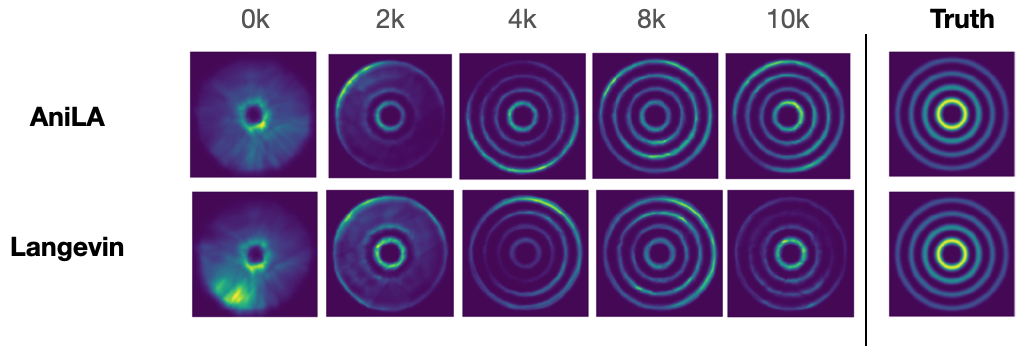
\includegraphics[width=0.8\textwidth]{figs/rings}
\caption{(Rings Toy Dataset) }
\label{fig:results}
\end{center}
\end{figure}


\subsection{Flowers Dataset}

\begin{figure}[H]
    \begin{center}
        \mbox{
        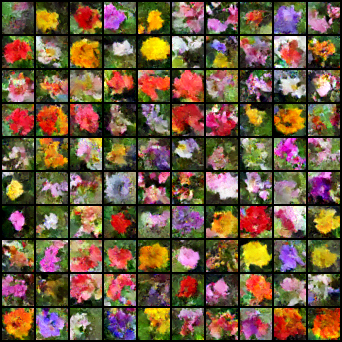
\includegraphics[width=2in]{figs/flowerslangevin}
        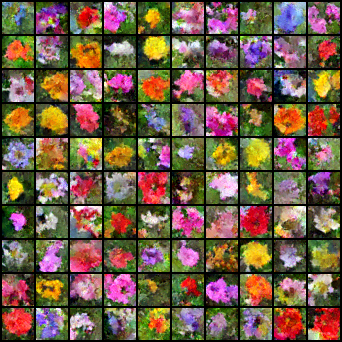
\includegraphics[width=2in]{figs/flowersanila}
        }
    \end{center}
    \vspace{-0.1in}
	\caption{(Flowers Dataset). Left: Langevin Method. Right: AniLA method. After 100k iterations.}
	\label{fig:flowers}
\end{figure}

\subsection{CIFAR Dataset}



\begin{figure}[H]
    \begin{center}
        \mbox{
        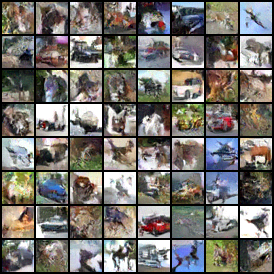
\includegraphics[width=2in]{figs/cifarlangevin}
        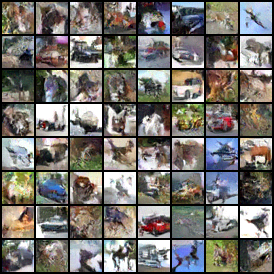
\includegraphics[width=2in]{figs/cifarlangevin}
        }
    \end{center}
    \vspace{-0.1in}
	\caption{(CIFAR Dataset). Left: Langevin Method. Right: AniLA method. After 100k iterations.}
	\label{fig:cifar}
\end{figure}


\section{Conclusion}\label{sec:conclusion}

\newpage

\bibliographystyle{plainnat}
\bibliography{ref}


\end{document} 